\documentclass{article}

% Gives us lovely headers
\usepackage{fancyhdr}
% Means you don't have to put \\ to start a new line.
\usepackage[parfill]{parskip}
% For including pictures
\usepackage{graphicx}
% For line brakes in tables
\usepackage{tabularx}
% For the split environment
\usepackage{amsmath}

\begin{document}
% Meta
\author{Chris Williamson, Todd Davies}
\title{COMP15111 Notes}
\rhead{COMP15111 Notes}

\maketitle
\tableofcontents
\newpage

\section{Lecture 1: Introduction}
\subsection{A Computational Model}
The simplest, earliest, commonest, most important computational model is the \textbf{Von-Neumann Imperative Procedural Computer Model}

According to this model, a computer can:
\begin{enumerate}
	\item Store information
	\item Manipulate the stored information
	\item Make decisions depending on the stored information
\end{enumerate}

\subsection{Simple View Of A Computer}
The simplest model of a computer can be represented as:

\[
	Memory \Leftrightarrow Bus \Leftrightarrow Processor
\]

\subsubsection{Memory}
Memory is a set of locations which can hold information, such as numbers(or programs). Each memory location has a unique (numerical) address, and there are typically thousands of millions of different locations. There are various ways of depicting memory; a common one is a 'hex dump' that often looks something like this: \marginpar{\raggedright Run the command {\it hexdump} to generate hexdumps.}

\begin{tabular}{l l l}
	Address     &	Values (8 bit numbers)	&	Characters\\
	00000000	&	48 65 6c 6c 6f 0a		&	Hello.\\
\end{tabular}

Each item that is in the memory has a unique address.

\subsubsection{Bus}
A bus is a bidirectional communication path. It is able to transmit addresses and numbers between components inside the computer.

\subsubsection{Processor}
The processor obeys a sequence of instructions, commonly referred to as a program.
Historically the processor was often referred to as a CPU, however, this is inappropriate nowadays since typical processors consist of several processing cores.

\subsection{Three-address instructions}
Every kind of processor has a different set of instructions, real world examples include: Pentium, ARM and others

Each three-address instruction:
\begin{enumerate}
	\item Copies the values from any two memory locations and sends them to the processor (source operands)
	\item Copies some operation e.g. adds the copied numbers together
	\item Copies the result back from the processor into a third memory location (destination operand)
\end{enumerate}

For example, if we wanted to convert the Java code $sum = a + b;$ into a three-address instruction we would:
\begin{enumerate}
	\item Identify the two {\it source operands}: $a$ holds 2, $b$ holds 3
	\item Perform the {\it operation}: 2 + 3 = 5
	\item Let the variable $sum$ equal the answer 5. This is the {\it destination operand}
\end{enumerate}

\subsubsection{Three address example}
{\bf Question:} Convert the Java code {\it product = c * d;} into the three-address style and draw a two box view of it.

First we need to re-write the Java code in the three-address style:
\[
	product \leftarrow c * d
\]
Now we can draw the box view of it:

\begin{figure}[ht!]
	\centering
	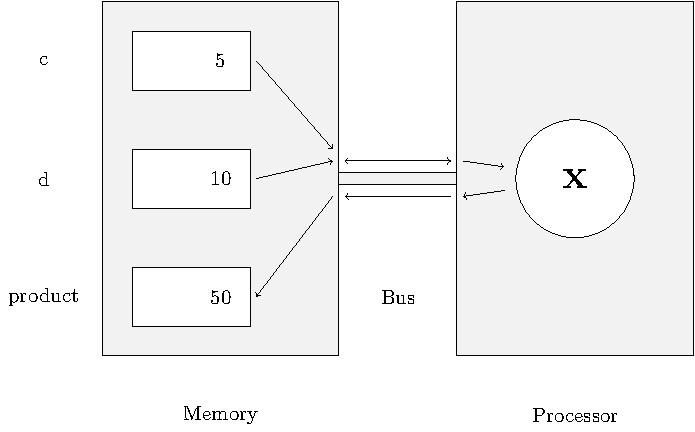
\includegraphics[width=90mm]{two_box_model_diagram.pdf}
	\caption{An example of the two box model}
	\label{overflow}
\end{figure}

\subsubsection{Memory bottleneck}
Most processors can process instructions faster than they can be fed by memory. Each instruction in the three-address cycle requires four memory cycles:

\begin{enumerate}
    \item Fetch the instruction
    \item Read the first operand
    \item Read the second operand
    \item Write the result to memory
\end{enumerate}

Each of these memory cycles could take hundreds of processor clock cycles to complete, and so in this time the processor would be doing nothing. However, most modern processors employ a {\it cache} to temporarily store commonly accessed memory locations, and so avoid some of the memory cycles. 

\subsection{Registers}
Registers are very small amounts of storage build into a processor. Since they are inside the processor data doesn't need to be transferred over the bus, and so they are very fast. Registers are used instead of the main memory which speeds up program execution.

Each register can only hold one value and each processor will only generally have a few dozen registers (e.g. ARM has sixteen).

\subsection{Instruction Styles}

\subsubsection{One address}
The one address style can only use up to one memory location in each instruction, all other operands must be registers. An example may be:

\[
    R1 \leftarrow R0 + \textrm{\it memory location}
\]

\subsubsection{Load-store}
The load-store style cannot perform operations on memory locations at all. Instead, values from memory must be loaded into a registers before the operation takes place and then the operation can be performed on the registers. Following the operation, the result must be stored back into memory again.

\[
	\begin{split}
	    R1 &\leftarrow \textrm{\it memory location}\\
		R1 &\leftarrow R0 + R1\\
	    \textrm{\it memory location} &\leftarrow R1
    \end{split}
\]

This means that we need extra instructions to do stuff with memory locations:
\begin{enumerate}
	\item \textbf{Load} the value from memory into a register before the operation.
	\item \textbf{Store} the value in the register back to memory after the operation.
\end{enumerate}

For example, the Java code {\it Sum = a + b + c;} would be run as:

\begin{center}
    \begin{tabular}{l l l r}
        R1 & $\leftarrow$ & a & (i.e. load from a)\\
        R2 & $\leftarrow$ & b & (i.e. load from b)\\
        R3 & $\leftarrow$ & R1 + R2 & (i.e. a+b)\\
        R4 & $\leftarrow$ & c & (i.e. load from c)\\
        R5 & $\leftarrow$ & R3 + R4  & (i.e. (a+b)+c)\\
        Sum & $\rightarrow$ & R5 & (i.e. store to sum)\\
    \end{tabular}
\end{center}

You can see that the load-store style favours lots of very simple, very fast instructions.

\section{Lecture 2}
Computers obey programs which are sequences of instructions. Instructions are coded as values in memory. The sequences are held in memory adjacent memory locations. Values in memory can be interpreted as you please, from numbers to text, to images or anything really!

Any given set of binary digits can be read as a decimal number, but not always as text, so values in memory are often represented as numbers for convenience.

\subsection{Assembly Language}
Assembly language is a means of representing machine instructions in a human readable form.

Each type of processor has its own assembly language (since each language is specific to a partial architecture) but they typically have a lot in common:

\begin{itemize}
	\item A mnemonic, that specifies the type of operation
	\item A destination, such as a register or memory location
	\item And one or more sources that may be registers or memory locations.
	\item Possibly with a comment too which will help programmers understand what's happening and aren't interpreted by the assembler.
\end{itemize}

When a program has been written in assembler, it must be {\it assembled} by an {\it assembler} to run it.

\subsection{ARM instructions}

ARM has many instructions but we only need three categories:

\begin{itemize}
	\item Memory operations that move data between the memory and the registers.
	\item Processing operations that perform calculations using value already in registers.
	\item Control flow instructions are used to make decisions, repeat operations etc.
\end{itemize}

\subsection{Transferring data between registers and memory}

Memory operations load a register from the memory or store a register value to the memory.

For example, $a$ into register 1 ($R1 \leftarrow a$) we would write:
{\tt LDR R1, a}

Or to store the value in register 5 into $sum$ ($sum \leftarrow R5$):
{\tt STR R5, sum}

In these examples, $a$ and $sum$ are aliases for the addresses of memory locations.

\subsection{ARM processing instructions}

ARM has many different instructions to perform operations such as addition, subtraction and multiplication.

The syntax for such operations is usually:

\begin{verbatim}
	[operand]	[destination register]	[register 1]	[register 2]
\end{verbatim}

For example, to add two numbers together, we might write:

\begin{verbatim}
	ADD R2, R0, R1
\end{verbatim}

This will add the value of R0 to the value of R1 and store it in R2.

\subsection{ARM control instructions}

The most common control instruction is the branch. Similar to \texttt{GOTO} in other languages, a branch will change the PC register (see section~\ref{subsec:pc}) to another value so the order of execution of the program is changed.

% TODO: change (coming up later) to the actual section when it's written

Branches can be made to be conditional by appending a conditional operator (coming up later) on to the command.

The syntax is something like:

\begin{verbatim}
	B[conditional operator]	[branch name]
\end{verbatim}

Some examples of different conditional operators are:

\begin{tabularx}{\textwidth}{l X}
	{\bf Command} & {\bf Function}\\
	\texttt{B} & Branches to a different location in the code.\\
	\texttt{BNE} & Branches, but only if the previous condition was false.\\
	\texttt{BEQ} & Branches, but only if the previous condition was true.\\
\end{tabularx}

\subsection{Stored programs and the Program Counter}
\label{subsec:pc}

A computer can make decisions, and choose which instructions to obey next depending upon the results of those decisions. A {\bf Program Counter} (PC) register is used to hold the memory address of the next instruction to be executed. ARM uses register 15 as its PC.

\subsection{Fetch-Execute Cycle}

The processor must first fetch instructions from memory before it can execute them. This is called the fetch-execute cycle, and it involves:

\begin{enumerate}
	\item \textbf{Fetch}: copy the instruction, pointed to by the PC, from memory and set PC to point to the next instruction
	\item \textbf{Execute}:  obey the instruction (exactly as before)
	\item Repeat.
\end{enumerate}

In ARM, the PC starts with a values of \texttt{0x00000000} when the program is initially run. On each cycle of the Fetch-Execute cycle, the PC is incremented by 4, since instructions each occupy 4 memory locations.

\subsection{Decision Making}

In order to make decisions, the computer mustn't just execute instructions one after the other in a linear manner. Instead, branches must be used to change the sequence of instructions to be executed.

In order to perform a conditional branch, we must first perform a compare command to perform the comparison before we do the branch.

\subsubsection{An example}

If we wanted to do a $£1$ discount on a shopping list if the price was over $£20$, we would do the following:

\begin{verbatim}
			LDR	R0, total	; Load the total price into R0
	
			CMP	R0, #20		; Compare R0 and 20 (the literal)
			BLT	nodiscount	; If the price is too low, then don't discount
			SUB	R0, #1		; Deduct £1
			STR	R0, total	; Store the result back into memory

nodiscount	SVC	2			; Finish

total 		DEFW	25		; Lets say the total is $25
\end{verbatim}

\subsection{Allocating memory}

The \texttt{DEFW} (define word) operation puts a value in memory before the program is run. Any define operation is executed before the program is run.

The actual memory location that is used to store the value isn't known to the running program, however, an {\it alias} is attached to the memory location by the programmer and the memory location can be referenced through that.

The syntax for the \texttt{DEFW} command is as follows:

\begin{verbatim}
myage	DEFW	18
\end{verbatim}

Where {\tt myage} is the alias and {\tt 18} is the value.

\section{Lecture 7: Addresses and Addressing}
When a processor references memory it needs to produce an address.

The address needs the same number of bits as the memory address. i.e. 32 in ARM

addressing modes - mechanisms for generating addresses

\subsection{Direct Addressing}
Direct addressing is a mode where the address is simply contained within the instruction.

This requires an instruction longer than the address size which is a problem because ARMs maximum bit length is 32.

So far, we assumed that direct addressing uses LDR/STR instructions, for example:

\begin{center}
    \begin{tabular}{l l l}
        LDR & R0, & b\\
        LDR & R1, & c\\
        ADD & R0, & R0, R2\\
        STR & R0, & a \\
    \end{tabular}
\end{center}

This looks like direct addressing but on ARM it's 'faked' by the assembler as a pseudo-instruction

\subsubsection{Problems with direct addressing}
ARM: both instructions and addresses are 32 bits, but the instruction also specifies operation so it can't contain every possible address.

Solution: allow a register to contain an address, use the address in the register to do loads and stores.

This is {\bf Register Indirect Addressing}

\subsection{Register Indirect Addressing}
The address is held in the register

It takes only a few bits to select a register (4 bits in the case of ARM R0-R15)

A register can (typically) hold an arbitrary address (32 bits in the case of ARM)

ARM has register indirect addressing

\paragraph{Example}
loading a register from a memory location: LDR R0, b

Could be done using register indirect addressing:

\begin{center}
    \begin{tabular}{l l l l}
        ADR & R2, & b & move the {\bf address} of b into R2\\
        LDR & R0, & [R2] & use address in R2 to fetch the {\bf value} of b\\
    \end{tabular}
\end{center}

This is still a bit limited - addresses are:

\begin{itemize}
  \item range limited (within ADR 'instruction')
  \item fixed
\end{itemize}

but:

\begin{itemize}
  \item ADRL pseudo-op allows larger range (at a price)
  \item having addresses a variable once it is often used again
  \item variable are usually 'near' each other
\end{itemize}

\subsubsection{Address Arithmetic}
We can operate on registers, so we can:

\begin{itemize}
  \item store/load/move addresses
  \item do arithmetic to calculate addresses
\end{itemize}

Rather than use e.g. extra ADD instructions, we often use {\bf Base + Offset Addressing} - address addition done within the operand.

We have actually been using this all along: Base = PC register.

\section{Offset Addressing}
In offset addressing the address is calculated from a register value and a number.

The register specifier is just a few bits, The offset can be 'fairly small'.

With one register 'pointer' any of several variables in nearby addresses may be addressed.

ARM allows offsets of 12 bits in LDR/STR

These bits can be added or subtracted, for example:

\begin{center}
    \begin{tabular}{l l l}
        {\tt LDR} & R0, & [R1, \#8] \\
        STR & R3, & [R6, \#-0x240]\\
        LDR & R7, & [R2, \#short-constant]
    \end{tabular}
\end{center}

This provides a range of $\pm$ ~4 kilobytes around a 'base' register

In practice this method is adequate for most purposes. 
\end{document}

